\subsubsection{Génération du signal NRZ}
Dans un premier temps, nous générons aléatoirement un signal binaire composé de \textcolor{Red}{\lstinline{Nb_bit = 100} bits}.

\begin{lstlisting}[caption=Génération aléatoire d'un signal binaire]
Nb_bit = 100;
Donnee = randi([0, 1], 1, Nb_bit);
\end{lstlisting}

Selon la norme V21, nous voulons transmettre le signal à \textcolor{Red}{\lstinline{Debit = 300} $bits\cdot s^{-1}$}.
   De plus, nous avons une fréquence d'échantillonnage définie à \textcolor{Red}{\lstinline{Fe = 48000} Hz}.
   Nous en dédsuisons le nombre \lstinline{Ns} d'échantillons à générer par bit (0 ou 1).


   \begin{lstlisting}[caption=Détermination du nombre $N_s$ d'échantillons]
Debit = 300;
Fe = 48000; Te = 1 / Fe;
Ts = 1 / Debit;
Ns = round(Ts / Te);
\end{lstlisting}

   On peut ainsi générer le signal NRZ, et le tracer (Figure \ref{fig : nrz}).

   \begin{lstlisting}[caption=Génération du signal NRZ]
NRZ = kron(Donnee, ones(1, Ns));
t = (0:Te:(Ns * Nb_bit - 1) * Te);
\end{lstlisting}


   \begin{figure}[ht!]
      \centering
      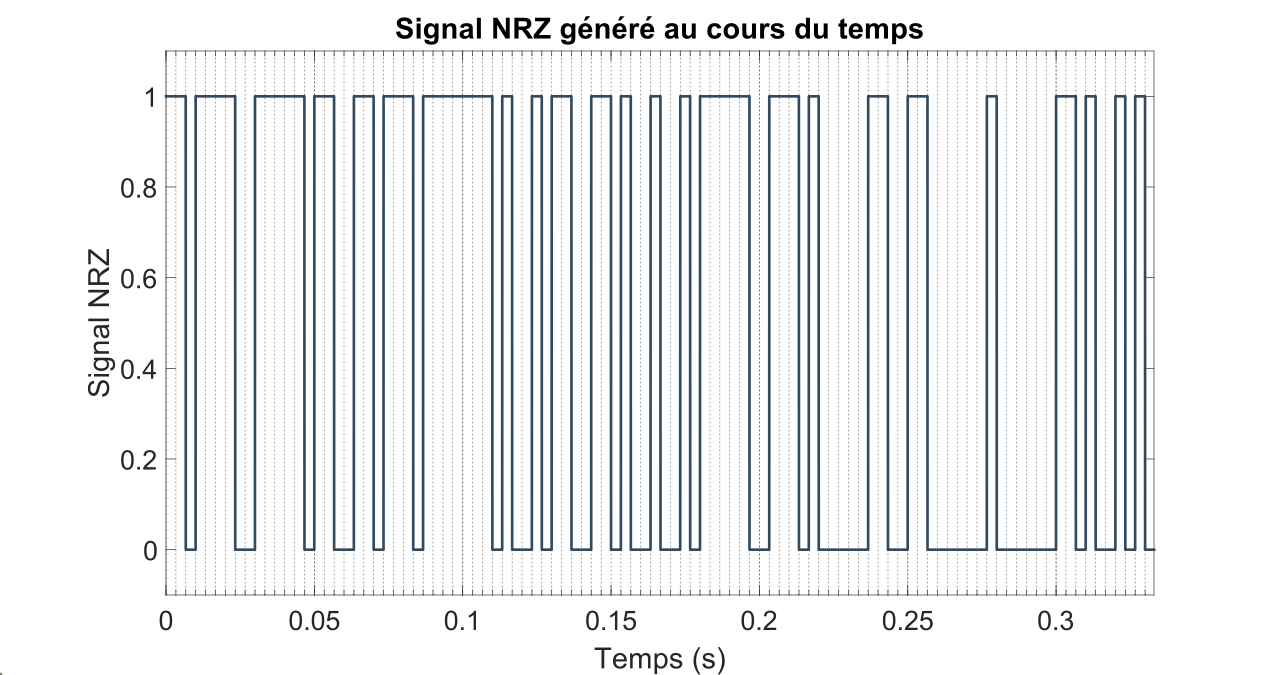
\includegraphics[scale=0.4]{partie-2/sous-partie-1/2.1.1.1.png}
      \caption{Signal généré NRZ \label{fig : nrz}}
   \end{figure}

   Grâce à la grille, on peut compter par exemple 15 bits en 0.05 secondes, soit un débit de $15\times \frac{1}{0.05} = 300 bit\cdot s^{-1}$.
Nous pouvons de plus estimer la densité spectrale de ce signal NRZ en utilisant la fonction \lstinline{periodogram} de matlab.

\begin{lstlisting}[]
periodogram(NRZ, [], length(NRZ),1/Ts)
\end{lstlisting}

\begin{figure}[ht!]
   \centering
   \includegraphics[scale=0.4]{partie-2/sous-partie-1/2.1.1.3.png}
   \caption{Periodogramme de NRZ \label{fig : p_nrz}}
\end{figure}

\subsubsection{Génération du signal modulé en fréquence}
Nous allons maintenant générer le signal modulé en fréquence selon l'équation suivante :
\[
   x(t) = (1-NRZ(t)) \times cos(2\pi F_{0}t+\phi_{0}) + NRZ(t)\times cos(2\pi F_{1}t+\phi_{1})
\]
Comme nous devrons d'abord faire un filtrage (après bruitage), pour l'instant, les fréquences $F_{0}$ et $F_{1}$ sont éloignées l'une de l'autre :
\[
   \left\{
   \begin{array}{r c l}
      F_0 & = & 6  000  Hz \\
      F_1 & = & 2  000  Hz \\
   \end{array}
   \right.\newline
\]
\begin{lstlisting}[caption=Génération du signal modulé, label=code4]
F0 = 6000; F1 = 2000;
phi0 = rand * 2 * pi;
phi1 = rand * 2 * pi;
x = (1 - NRZ) .* cos(2 * pi * F0 * t + phi0) + NRZ .* cos(2 * pi * F1 * t + phi1);
plot(t, x);
\end{lstlisting}
\begin{figure}[ht!]
   \centering
   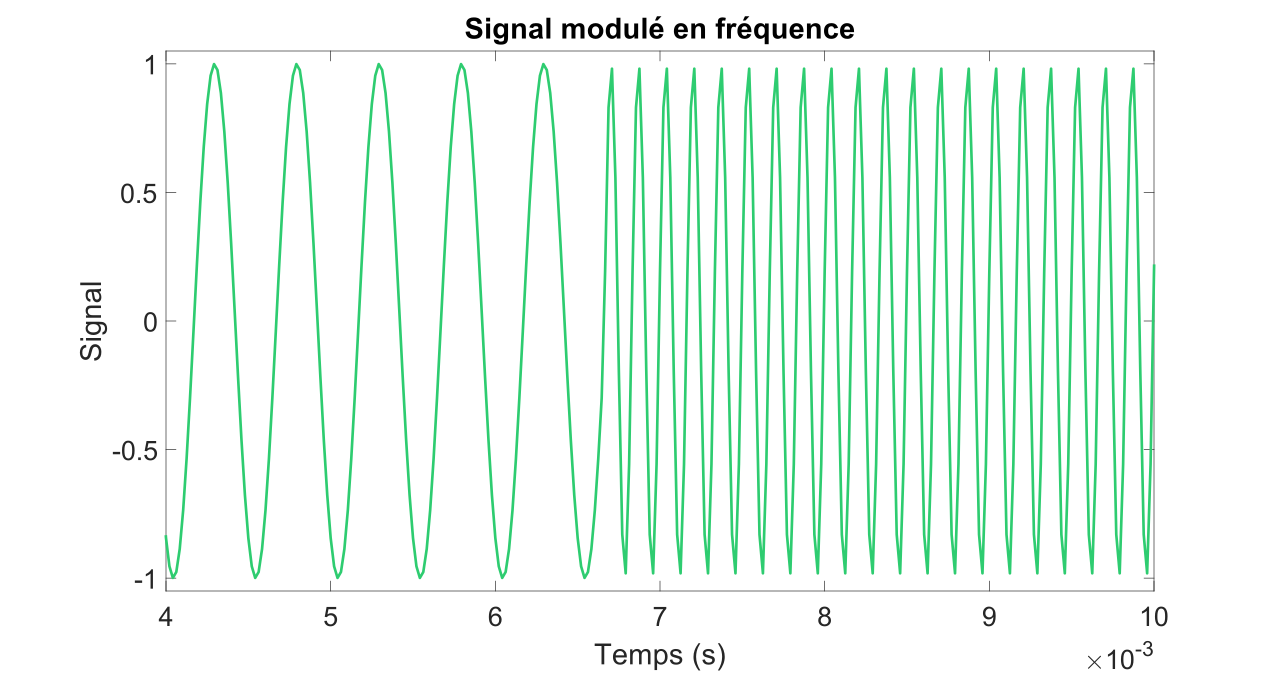
\includegraphics[scale=0.4]{partie-2/sous-partie-1/2.1.2.1.png}
   \caption{Signal modulé en fréquence \label{fig : signal-module}}
\end{figure}
Sur la Figure \ref{fig : signal-module} nous avons zoomé pour bien voir la modulation en fréquence : sur l'intervalle $[4\cdot 10^{-3} ; 6,6\cdot 10^{-3}]$,
nous retrouvons la fréquence $F_1$, et sur l'intervalle $[6,6\cdot 10^{-3} ; 10\cdot 10^{-3}]$, la fréquence $F_0$.
Calculons la densité spectrale de puissance théorique de ce signal.
\begin{dinglist}{111}
   \item \textbf{Type de signal.} $\phi_0$ et $\phi_1$ sont des variables aléatoires indépendantes. On se penche donc vers un signal aléatoire. Montrons qu'il est stationnaire :
   \[
      \left\{
      \begin{array}{rcl}
         m_x       & = & E[x(t)]            \\
         R_x(\tau) & = & E[x(t)x^*(t-\tau)] \\
      \end{array}
      \right.
   \]
   Notons que $NRZ(t)$, $\phi_0$ et $\phi_1$ sont indépendantes, donc :
   \[
      \left\{
      \begin{array}{rcl}
         m_x       & = & E[cos(2\pi F_0 t+ \phi_0)] - E[NRZ(t)] \times E[cos(2\pi F_0 t+ \phi_0)] + E[NRZ(t)] \times E[cos(2 \pi F_1 t + \phi_1)] \\
         R_x(\tau) & = & ...                                                                                                                      \\
      \end{array}
      \right.
   \]
   \[
      \iff
      \left\{
      \begin{array}{rcl}
         m_x       & = & 0                                                                     \\
         R_x(\tau) & = & R_{NRZ}(\tau)\times\frac{1}{2}(cos(2\pi F_1\tau) - cos(2\pi F_0\tau)) \\
      \end{array}
      \right.
   \]
   Ainsi, $m_x$ et $R_x$ ne dépendent pas du temps. Alors, $x(t)$ est stationnaire.
   \item  \textbf{Densité spectrale de puissance.}
   \[S_x(f) = TF[R_x(\tau)]\]
   \[S_x(f) = \frac{1}{4}(S_{NRZ}(f-f_1)+S_{NRZ}(f+f_1) - S_{NRZ}(f-f_0)-S_{NRZ}(f+f_0))\]
\end{dinglist}
De la même manière que nous avons estimé la densité spectrale du signal NRZ, nous calculons celle du signal $x(t)$.